
\begin{equation}
    \vec{B} - \vec{A} = \myvec{-3\\-5\\-3}, \vec{C} - \vec{A} = \myvec{3\\5\\13}
\end{equation}
Forming the matrix 
\begin{align}
    \vec{M} &= \myvec{
    \vec{B} -  \vec{A} & \vec{C} - \vec{A}\\
    }^\top\\
    &= \myvec{
    -3 & -5 & -3\\
    3 & 5 & 3}
\end{align}
Using matrix transformation,
\begin{align}
 \vec{M} = \myvec{
    -3 & -5 & -3\\
    3 & 5 & 3}
    \xleftrightarrow{\text{$R_2$}\rightarrow{\text{$R_2 + R_1$ }}}
 \myvec{
 -3 & -5 & -3\\
 0 & 0 & 0}\
\end{align}
\begin{equation}
   \implies rank(\vec{M}) = 1 
\end{equation}
Thus $\vec{A}$, $\vec{B}$ and $\vec{C}$ are collinear as can be seen from Fig. \ref{aug/2/14/plt}
\begin{figure}[!h]
    \centering
    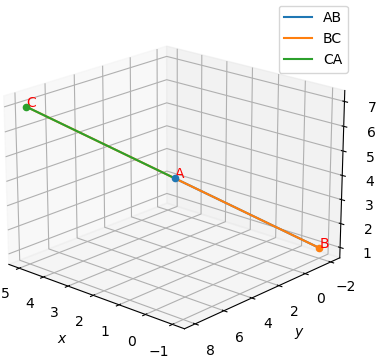
\includegraphics[width=\columnwidth]{solutions/aug/2/14/Figures/plot.png}
    \caption{Plot of the line}
    \label{aug/2/14/plt}
    \end{figure}